%%% Hlavní soubor. Zde se definují základní parametry a odkazuje se na ostatní části. %%%

%% Verze pro jednostranný tisk:
% Okraje: levý 40mm, pravý 25mm, horní a dolní 25mm
% (ale pozor, LaTeX si sám přidává 1in)
\documentclass[12pt,a4paper]{report}
\setlength\textwidth{145mm}
\setlength\textheight{247mm}
\setlength\oddsidemargin{15mm}
\setlength\evensidemargin{15mm}
\setlength\topmargin{0mm}
\setlength\headsep{0mm}
\setlength\headheight{0mm}
% \openright zařídí, aby následující text začínal na pravé straně knihy
\let\openright=\clearpage

%% Pokud tiskneme oboustranně:
% \documentclass[12pt,a4paper,twoside,openright]{report}
% \setlength\textwidth{145mm}
% \setlength\textheight{247mm}
% \setlength\oddsidemargin{14.2mm}
% \setlength\evensidemargin{0mm}
% \setlength\topmargin{0mm}
% \setlength\headsep{0mm}
% \setlength\headheight{0mm}
% \let\openright=\cleardoublepage

%% Vytváříme PDF/A-2u
\usepackage[a-2u]{pdfx}

%% Přepneme na českou sazbu a fonty Latin Modern
\usepackage[czech]{babel}
\usepackage{lmodern}
\usepackage[T1]{fontenc}
\usepackage{textcomp}

%% Použité kódování znaků: obvykle latin2, cp1250 nebo utf8:
\usepackage[utf8]{inputenc}

%%% Další užitečné balíčky (jsou součástí běžných distribucí LaTeXu)
\usepackage{amsmath}        % rozšíření pro sazbu matematiky
\usepackage{amsfonts}       % matematické fonty
\usepackage{amsthm}         % sazba vět, definic apod.
\usepackage{bbding}         % balíček s nejrůznějšími symboly
			    			% (čtverečky, hvězdičky, tužtičky, nůžtičky, ...)
\usepackage{bm}             % tučné symboly (příkaz \bm)
\usepackage{graphicx}       % vkládání obrázků
\usepackage{fancyvrb}       % vylepšené prostředí pro strojové písmo
\usepackage{indentfirst}    % zavede odsazení 1. odstavce kapitoly
\usepackage{natbib}         % zajišťuje možnost odkazovat na literaturu
							% stylem AUTOR (ROK), resp. AUTOR [ČÍSLO]
\usepackage[nottoc]{tocbibind} % zajistí přidání seznamu literatury,
                            % obrázků a tabulek do obsahu
\usepackage{icomma}         % inteligetní čárka v matematickém módu
\usepackage{dcolumn}        % lepší zarovnání sloupců v tabulkách
\usepackage{booktabs}       % lepší vodorovné linky v tabulkách
\usepackage{paralist}       % lepší enumerate a itemize
\usepackage{xcolor}         % barevná sazba


\usepackage{wrapfig}         % obrázek plující vedle textu
\usepackage{multicol}        % sloupečky
\usepackage{listings}		 % highlighting kódu
\hyphenpenalty 5000
\exhyphenpenalty 5000
\usepackage[font=scriptsize, skip=1pt]{caption}		% pro seznam obrázku a tabulek
\DeclareCaptionLabelSeparator{bar}{\space\textbar\space}
\captionsetup{labelsep=bar}
\addto\captionsczech{\renewcommand{\figurename}{Obr.}}


\usepackage[light,scaled=0.85]{roboto-mono}


%%% Údaje o práci

% Název práce v jazyce práce (přesně podle zadání)
\def\NazevPrace{Softwarové řešení digitálních archivů}

% Název práce v angličtině
\def\NazevPraceEN{Software solution for digital archives}

% Jméno autora
\def\AutorPrace{David Nápravník}

% Rok odevzdání
\def\RokOdevzdani{2021}

% Název katedry nebo ústavu, kde byla práce oficiálně zadána
% (dle Organizační struktury MFF UK, případně plný název pracoviště mimo MFF)
\def\Katedra{Katedra teoretické informatiky a matematické logiky}
\def\KatedraEN{Department of Theoretical Computer Science and Mathematical Logic}

% Jedná se o katedru (department) nebo o ústav (institute)?
\def\TypPracoviste{Katedra}
\def\TypPracovisteEN{Department}

% Vedoucí práce: Jméno a příjmení s~tituly
\def\Vedouci{Mgr. Kateřina Macková}

% Pracoviště vedoucího (opět dle Organizační struktury MFF)
\def\KatedraVedouciho{Ústav formální a aplikované lingvistiky}
\def\KatedraVedoucihoEN{Institute of Formal and Applied Linguistics}

% Studijní program a obor
\def\StudijniProgram{Informatika (B1801)}
\def\StudijniObor{IPSS (1801R048)}

% Nepovinné poděkování (vedoucímu práce, konzultantovi, tomu, kdo
% zapůjčil software, literaturu apod.)
\def\Podekovani{
TODO Poděkovaní:\\
Petra Hoffmannová\\
Kateřina Macková\\
Anička Yaghobová\\
Monika Bošániová\\
}

% Abstrakt (doporučený rozsah cca 80-200 slov; nejedná se o zadání práce)
\def\Abstrakt{%
Za použití moderních webových a databázových technologií byla vyvynuta aplikace
jako náhrada za zastaralé knihovní systémy. 
Byly snížemy požadavky na výkon serveru a síťového rozhraní. 
Uživatel tak má intuitivní rychlou webovou aplikaci,
jež kombinuje knihovní a redakční systém a další moduly, jež
nějakým způsobem zobrazují historické objekty, jako jsou mapy nebo 3D modely.
Vývojáři a automatizované systémy pak mají přístup k uchovávaným datům
přes jednoduché a rychle API a umožní jim tak data napojit na své systémy.
}
\def\AbstraktEN{%
TODO Abstrakt en
}

% 3 až 5 klíčových slov (doporučeno), každé uzavřeno ve složených závorkách
\def\KlicovaSlova{%
{digitální archiv}, {web}, {databáze}
}
\def\KlicovaSlovaEN{%
{digital archive} {web} {database}
}

%% Balíček hyperref, kterým jdou vyrábět klikací odkazy v PDF,
%% ale hlavně ho používáme k uložení metadat do PDF (včetně obsahu).
%% Většinu nastavítek přednastaví balíček pdfx.
\hypersetup{unicode}
\hypersetup{breaklinks=true}

%% Definice různých užitečných maker (viz popis uvnitř souboru)
%%% Tento soubor obsahuje definice různých užitečných maker a prostředí %%%
%%% Další makra připisujte sem, ať nepřekáží v ostatních souborech.     %%%

%%% Drobné úpravy stylu

% Tato makra přesvědčují mírně ošklivým trikem LaTeX, aby hlavičky kapitol
% sázel příčetněji a nevynechával nad nimi spoustu místa. Směle ignorujte.
\makeatletter
\def\@makechapterhead#1{
  {\parindent \z@ \raggedright \normalfont
   \Huge\bfseries \thechapter. #1
   \par\nobreak
   \vskip 20\p@
}}
\def\@makeschapterhead#1{
  {\parindent \z@ \raggedright \normalfont
   \Huge\bfseries #1
   \par\nobreak
   \vskip 20\p@
}}
\makeatother

% Toto makro definuje kapitolu, která není očíslovaná, ale je uvedena v obsahu.
\def\chapwithtoc#1{
\chapter*{#1}
\addcontentsline{toc}{chapter}{#1}
}

% Trochu volnější nastavení dělení slov, než je default.
\lefthyphenmin=2
\righthyphenmin=2

% Zapne černé "slimáky" na koncích řádků, které přetekly, abychom si
% jich lépe všimli.
\overfullrule=1mm

%%% Makra pro definice, věty, tvrzení, příklady, ... (vyžaduje baliček amsthm)

\theoremstyle{plain}
\newtheorem{veta}{Věta}
\newtheorem{lemma}[veta]{Lemma}
\newtheorem{tvrz}[veta]{Tvrzení}

\theoremstyle{plain}
\newtheorem{definice}{Definice}

\theoremstyle{remark}
\newtheorem*{dusl}{Důsledek}
\newtheorem*{pozn}{Poznámka}
\newtheorem*{prikl}{Příklad}

%%% Prostředí pro důkazy

\newenvironment{dukaz}{
  \par\medskip\noindent
  \textit{Důkaz}.
}{
\newline
\rightline{$\qedsymbol$}
}

%%% Prostředí pro sazbu kódu, případně vstupu/výstupu počítačových
%%% programů. (Vyžaduje balíček fancyvrb -- fancy verbatim.)

\DefineVerbatimEnvironment{code}{Verbatim}{fontsize=\small, frame=single}

%%% Prostor reálných, resp. přirozených čísel
\newcommand{\R}{\mathbb{R}}
\newcommand{\N}{\mathbb{N}}

%%% Užitečné operátory pro statistiku a pravděpodobnost
\DeclareMathOperator{\pr}{\textsf{P}}
\DeclareMathOperator{\E}{\textsf{E}\,}
\DeclareMathOperator{\var}{\textrm{var}}
\DeclareMathOperator{\sd}{\textrm{sd}}

%%% Příkaz pro transpozici vektoru/matice
\newcommand{\T}[1]{#1^\top}

%%% Vychytávky pro matematiku
\newcommand{\goto}{\rightarrow}
\newcommand{\gotop}{\stackrel{P}{\longrightarrow}}
\newcommand{\maon}[1]{o(n^{#1})}
\newcommand{\abs}[1]{\left|{#1}\right|}
\newcommand{\dint}{\int_0^\tau\!\!\int_0^\tau}
\newcommand{\isqr}[1]{\frac{1}{\sqrt{#1}}}

%%% Vychytávky pro tabulky
\newcommand{\pulrad}[1]{\raisebox{1.5ex}[0pt]{#1}}
\newcommand{\mc}[1]{\multicolumn{1}{c}{#1}}


%Define the listing package
\usepackage{color} %use color
\definecolor{mygreen}{rgb}{0,0.6,0}
\definecolor{mygray}{rgb}{0.5,0.5,0.5}
\definecolor{mymauve}{rgb}{0.58,0,0.82}
 
%Customize a bit the look
\lstset{ %
  backgroundcolor=\color{white}, % choose the background color; you must add \usepackage{color} or \usepackage{xcolor}
  basicstyle=\footnotesize, % the size of the fonts that are used for the code
  breakatwhitespace=false, % sets if automatic breaks should only happen at whitespace
  breaklines=true, % sets automatic line breaking
  captionpos=b, % sets the caption-position to bottom
  commentstyle=\color{mygreen}, % comment style
  deletekeywords={...}, % if you want to delete keywords from the given language
  escapeinside={\%*}{*)}, % if you want to add LaTeX within your code
  extendedchars=true, % lets you use non-ASCII characters; for 8-bits encodings only, does not work with UTF-8
  frame=none, % adds a frame around the code
  keepspaces=true, % keeps spaces in text, useful for keeping indentation of code (possibly needs columns=flexible)
  keywordstyle=\color{blue}, % keyword style
  % language=Octave, % the language of the code
  morekeywords={*,...}, % if you want to add more keywords to the set
  numbers=none, % where to put the line-numbers; possible values are (none, left, right)
  numbersep=5pt, % how far the line-numbers are from the code
  numberstyle=\tiny\color{mygray}, % the style that is used for the line-numbers
  rulecolor=\color{black}, % if not set, the frame-color may be changed on line-breaks within not-black text (e.g. comments (green here))
  showspaces=false, % show spaces everywhere adding particular underscores; it overrides 'showstringspaces'
  showstringspaces=false, % underline spaces within strings only
  showtabs=false, % show tabs within strings adding particular underscores
  stepnumber=1, % the step between two line-numbers. If it's 1, each line will be numbered
  stringstyle=\color{mymauve}, % string literal style
  tabsize=4, % sets default tabsize to 4 spaces
  title=\lstname % show the filename of files included with \lstinputlisting; also try caption instead of title
}
%END of listing package%
 
\definecolor{darkgray}{rgb}{.4,.4,.4}
\definecolor{purple}{rgb}{0.65, 0.12, 0.82}
 
%define Javascript language
\lstdefinelanguage{JavaScript}{
  keywords={then, let, await, break, case, catch, class, const, continue, debugger, default, delete, do, else, enum, export, extends, false, finally, for, function, if, import, in, instanceof, new, null, return, super, switch, this, throw, true, try, typeof, var, void, while, with, yield},
  keywordstyle=\color{blue}\bfseries,
  ndkeywords={JSON, fetch, console},
  ndkeywordstyle=\color{purple}\bfseries,
  identifierstyle=\color{black},
  sensitive=false,
  comment=[l]{//},
  morecomment=[s]{/*}{*/},
  commentstyle=\color{purple}\ttfamily,
  stringstyle=\color{red}\ttfamily,
  morestring=[b]',
  morestring=[b]"
}
 
\lstset{
  language=JavaScript,
  extendedchars=true,
  basicstyle=\footnotesize\ttfamily,
  showstringspaces=false,
  showspaces=false,
  numberstyle=\footnotesize,
  numbersep=9pt,
  tabsize=2,
  breaklines=true,
  showtabs=false,
  captionpos=b
}

%% Titulní strana a různé povinné informační strany
\begin{document}
%%% Titulní strana práce a další povinné informační strany

%%% Titulní strana práce

\pagestyle{empty}
\hypersetup{pageanchor=false}

\begin{center}

\centerline{\mbox{
\includegraphics[width=166mm]{img/logo-cs.pdf}}}

\vspace{-8mm}
\vfill

{\bf\Large BAKALÁŘSKÁ PRÁCE}

\vfill

{\LARGE\AutorPrace}

\vspace{15mm}

{\LARGE\bfseries\NazevPrace}

\vfill

\Katedra

\vfill

{
\centerline{\vbox{\halign{\hbox to 0.45\hsize{\hfil #}&\hskip 0.5em\parbox[t]{0.45\hsize}{\raggedright #}\cr
Vedoucí bakalářské práce:&\Vedouci \cr
\noalign{\vspace{2mm}}
Studijní program:&\StudijniProgram \cr
\noalign{\vspace{2mm}}
Studijní obor:&\StudijniObor \cr
}}}}

\vfill

% Zde doplňte rok
Praha \RokOdevzdani

\end{center}

\newpage

%%% Následuje vevázaný list -- kopie podepsaného "Zadání bakalářské práce".
%%% Toto zadání NENÍ součástí elektronické verze práce, nescanovat.

%%% Strana s čestným prohlášením k bakalářské práci

\openright
\hypersetup{pageanchor=true}
\pagestyle{plain}
\pagenumbering{roman}
\vglue 0pt plus 1fill

\noindent
Prohlašuji, že jsem tuto bakalářskou práci vypracoval(a) samostatně a výhradně
s~použitím citovaných pramenů, literatury a dalších odborných zdrojů.
Tato práce nebyla využita k získání jiného nebo stejného titulu.

\medskip\noindent
Beru na~vědomí, že se na moji práci vztahují práva a povinnosti vyplývající
ze zákona č. 121/2000 Sb., autorského zákona v~platném znění, zejména skutečnost,
že Univerzita Karlova má právo na~uzavření licenční smlouvy o~užití této
práce jako školního díla podle §60 odst. 1 autorského zákona.

\vspace{10mm}

\hbox{\hbox to 0.5\hsize{%
V \hbox to 6em{\dotfill} dne \hbox to 6em{\dotfill}
\hss}\hbox to 0.5\hsize{\dotfill\quad}}
\smallskip
\hbox{\hbox to 0.5\hsize{}\hbox to 0.5\hsize{\hfil Podpis autora\hfil}}

\vspace{20mm}
\newpage

%%% Poděkování

\openright

\noindent
\Podekovani

\newpage

%%% Povinná informační strana bakalářské práce

\openright

\vbox to 0.5\vsize{
\setlength\parindent{0mm}
\setlength\parskip{5mm}

Název práce:
\NazevPrace

Autor:
\AutorPrace

\TypPracoviste:
\Katedra

Vedoucí bakalářské práce:
\Vedouci, \KatedraVedouciho

Abstrakt:
\Abstrakt

Klíčová slova:
\KlicovaSlova

\vss}\nobreak\vbox to 0.49\vsize{
\setlength\parindent{0mm}
\setlength\parskip{5mm}

Title:
\NazevPraceEN

Author:
\AutorPrace

\TypPracovisteEN:
\KatedraEN

Supervisor:
\Vedouci, \KatedraVedoucihoEN

Abstract:
\AbstraktEN

Keywords:
\KlicovaSlovaEN

\vss}

\newpage

\openright
\pagestyle{plain}
\pagenumbering{arabic}
\setcounter{page}{1}


%%% Strana s automaticky generovaným obsahem bakalářské práce

\tableofcontents

%%% Jednotlivé kapitoly práce jsou pro přehlednost uloženy v samostatných souborech
\chapter{Úvod}
Cílem této práce bylo vytvoření webové aplikace pro správu historických
objektů jako jsou elektronické záznamy, odborné články, 3D modely a mapy
z oblasti Krkonoš. \\
Systém by měl být vytvořen tak, aby splnil požadavky ze
strany historického ústavu, který poskytl data a zároveň byl efektivnější
a rychlejší než stávající knihovní systémy.\\

\chapter{Analýza a požadavky}
Vybíráme jen z open source produktů, abychom mohli nahlédnout
do jejich kódu a lépe porozumět implementaci jejich komponent.
Lépe se pro takový systém vyvíjejí externí moduly, protože
obvykle mají o dost větší komunitu vývojářů a přispěvatelů.


\section{Požadavky na systém}
Systém bude přístupný jako webová aplikace skrze moderní webové prohlížeče.
Zadavatel bude moci přidávat, prohlížet, měnit a mazat metadata a k nim příslušné indexy.
Redaktor bude moci přidávat a měnit články a novinky na webu.
Uživatel bude moci vyhledat záznam podle několika různých kritérií a poté jej zobrazit,
též bude moci zobrazit příspěvky na webu, včetně novinek.
Externí programátoři budou moci k systému přistupovat přes API a získávat nebo měnit data. 


\section{Pro koho je systém určen}
Systém bude sloužit pro pracovníky historického ústavu jakožto pro zadavatele
a redaktory stránek této aplikace a bude uchovávat historická data z oblasti Krkonoš,
tak aby si je návštěvník případně vědecký pracovník mohl přehledně
zobrazit na jednom místě a případně si data i automaticky stahovat přes připravené API.
Zároveň systém obsahuje interaktivní moduly, jež budou k dispozici
návštěvníkům výstavy Pramenů Krkonoš, jako je hologram 3D modelu nebo
prohlížeč historických map.

\clearpage
\section{Existující produkty}
\subsection{KOHA}
\begin{wrapfigure}[7]{r}{0.25\textwidth}
	
\includegraphics[width=\linewidth]{img/KOHA_Logo.png}\\
	\caption[LOGO systému koha ze stránky \url{https://www.mainelibit.org/node/77}]{LOGO systému koha}
\end{wrapfigure}
Domovská stránka aplikace: \url{http://www.koha.cz/}\\
Koha je nejrozšířenější open source systém s širokou komunitou.
Byla vyvinuta na Novém Zélandu roku 2000.
Ale je stále udržovaná a stále rozšiřovaná
(nejnovější update je z konce roku 2020)
\\
Používá SQL databázi.
Je psaná v Perlu, na frontendu využívající javascript (ale není jej tolik).

\subsection{Evergreen}
\begin{wrapfigure}[3]{r}{0.3\textwidth}
	\centering
	
\includegraphics[width=\linewidth]{img/Evergreen_Logo.png}\\
	\caption[LOGO systému Evergreen ze stránky \url{https://eg-wiki.osvobozena-knihovna.cz/}]{LOGO systému Evergreen}
\end{wrapfigure}
Domovská stránka aplikace: \\\url{https://eg-wiki.osvobozena-knihovna.cz}\\
Další z řady knihovních systému.
Používán např Pedagogickou a Teologickou Fakultou v Praze.\\
Používá sql databázi, vykreslovaní probíhá na serveru a nemá uživatelsky přivětivé prostředí.

\subsection{SLIMS}
\begin{wrapfigure}[5]{r}{0.15\textwidth}
	
\includegraphics[width=\linewidth]{img/Slims_Logo.png}\\
	\caption[LOGO systému SLIMS ze stránky \url{https://slims.web.id/}]{LOGO systému SLIMS}
\end{wrapfigure}
Domovská stránka aplikace: \url{https://slims.web.id/}\\
Systém se základní funkcionalitou a přivětivým vzhledem.
Není v češtině. Není primárně určen jako knihovní systém, spíš je to univerzální
systém na cokoliv, proto není až tak efektivní a jeho nastavovaní
by zabralo mnoho času.

\subsection{Porovnání existujících systémů}
Evergreen a SLIMS jsou systémy, které potřebují silně vyškolenou osobu,
aby se o systém starala, narozdíl od systému KOHA, která je intuitivnější a
pro nové uživatele přívětivější, při zachovaní stejné, možná i lepši funkcionality.\\

\chapter{Návrh projektu}

\section{Výběr technologií}

\subsection{Frontend}
Ačkoliv se trendy v oblasti vývoje webových aplikací mění velmi rychle,
jednou z nejpodstatnějších změn, která přenesla vykreslování stránky
na stranu uživatele a tim se výrazně odlišila od dosavadních konceptů
vykreslujících stránku na straně serveru, se stala technologie
\textbf{Single page aplication}. Celá aplikace pak je v tomto duchu
implementována a přizpůsobena s důrazem na plynulost a rychlost aplikace.

\subsubsection{Single page aplication}
Single page aplication je technologie umožnující vykreslení jiné stránky,
bez nutnosti, posílaní requestu na server.
Uživatel si při prvním spuštění webu stáhne celý balíček webu a 
při opětovném načtení vetšinou sahá jen do své lokální cache.
JavaScriptová knihovna (v tomto případě React)
poté stránku překresluje při uživatelské interakci.
V případě nutnosti stažení / posílaní dat mezi serverem a uživatelem
(např. editace záznamu, nebo načtení existujícího záznamu)
se volá pouze request k API webové služby a tělo requestu obsahuje pouze
užitečné (ne-redundantní) informace. 


\subsubsection{React}
Knihovna React poskytuje single page aplication technologii.
Jedná se o dobře udržovanou knihovnu, jež byla vyvinuta Facebookem 
jakožto náhrada zastaralého konceptu renderovaní stránky na serveru.
Díky tomu servery nemusejí ztrácet výkon s každou změnou na stránce a
výkon k renderovaní se bere z PC uživatele.
Jádro této knihovny je velmi dobře optimalizované a poskytuje i řadu
debuggovacích nástrojů, což je pro větší projekty nepostradatelná výhoda.  


\subsubsection{Další možné technologie}
Běžnou praxí vykreslování dynamické stránky je její vykreslení na straně serveru,
jako to má např. velmi populární redakční systém WordPress (jež je psaný v jazyce PHP).
Takovýto system je dobře uživatelsky přivětivý, ale za cenu masivního nárůstu
potřebného serverového výkonu.
V případě implementace knihovního systému by to znamenalo vykreslovat
celou stránku (hlavičku, tělo i zápatí) na serveru,
na druhé straně single page aplication na serveru nic nevykresluje a
pouze minimalisticky posílá požadované informace.


\subsection{Backend}
Mít single page aplikaci na frontendu znamená, že na backendu musí existovat API,
od kterého bude frontend čerpat data.
Navíc zde potřebujeme i systém pro statické odesílaní balíku celé webové stránky.
V rámci udržitelnosti byl použit stejný jazyk JavaScript, jaký je na frontendu.
Knihovnou, která by umožňovala komplexní správu requestů a zároveň by byla
i na robustnějších projektech programátorsky přehledná, byla zvolena Express.js.

\subsubsection{Express.js}
Express.js poskytuje nejen odesílaní statických stránek,
což je potřeba při odesílání balíku s aplikací React, ale umí i
custom requesty, potřebné pro rozmanité API a také odesílaní a
lokální ukládaní statických souborů, jako jsou obrázky a word nebo pdf dokumenty.

\subsubsection{MongoDB}
MongoDB je databázový systém typu non-SQL.
Což primárně znamená, že data neuchovává v tabulkách, ale v tzv. schématech.
Což má mnoho výhod, z nichž největší je, že nekompletní záznamy nezabírají
svými nevyplněnými daty místo v DB a ukládá se opravdu jen to, co je potřeba.
Další výhodou je styl ukládaní dat a komunikace s DB.
Databáze si data uchovává ve formátu BSON (binární JSON rozšířený o datové typy).
O data si aplikace žádá pomoci query,
která je zcela odlišná od těch u SQL databází,
primárně se zde neposílá query ve formátu string ale jako JSON objekt,
díky čemuž např. nenastane známá SQL injection.
Znovu ve formátu JSON poté data vrací aplikaci.

\subsubsection{Další možné technologie}
Díky odděleni frontendu a backendu (narozdíl od např. WordPressu) je možné
na backend nasadit téměř cokoliv co umí posílat requesty.
Příkladem toho můžou být scripty v jazycích PHP, C\#, Python, nebo Perl.
Ale vzhledem k tomu, že jedním z modulů bude neuronová síť na pokročilé vyhledávaní,
vybírali jsme mezi jazyky Python a JavaScript, jakožto dvěma jazyky, které
mají velmi dobré knihovny pro práci s neuronovými sítěmi.

\section{Diagram systému}
\begin{figure}[H]
	\centering
	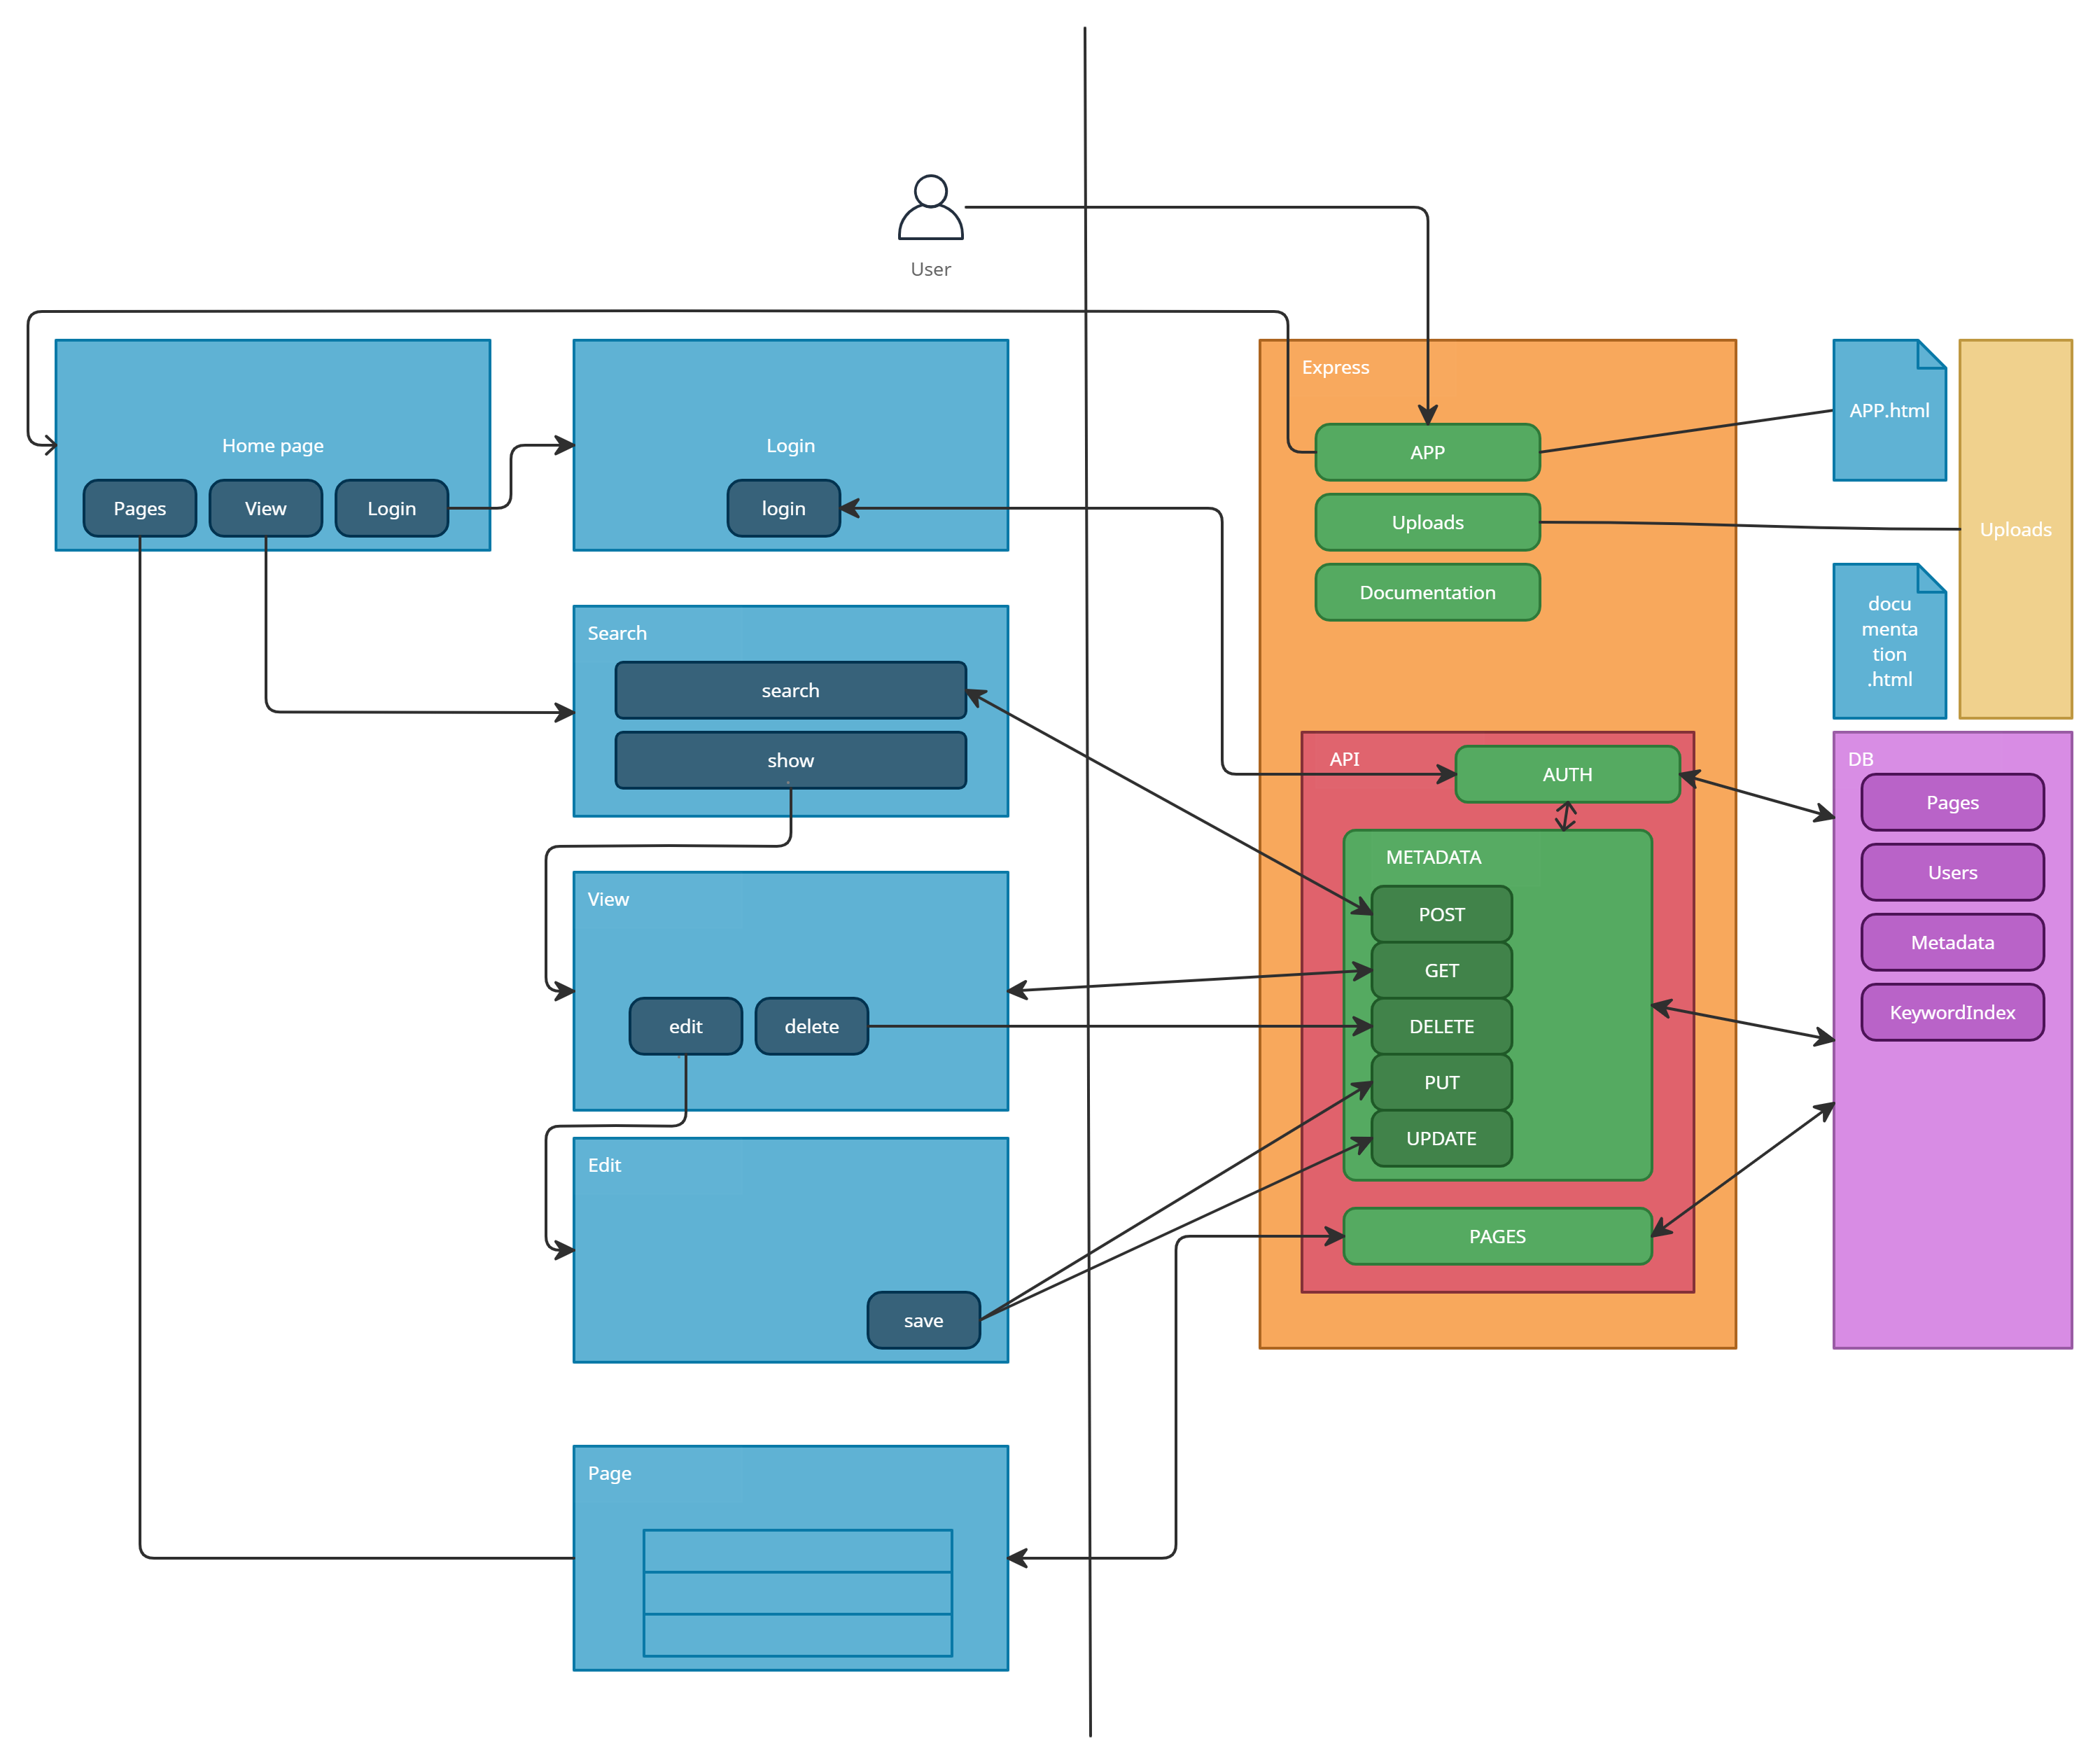
\includegraphics[angle=-90,origin=c,width=\linewidth]{img/diagram.png}
	\caption{Diagram systému}
\end{figure}

\chapter{implementace backendu}

\chapter{implementace frontendu}

\section{server}
\subsection{kompilace}
\subsection{npm}

\section{knihovny}
\subsection{React}
\subsection{Material-ui}
\subsection{i18n}
\subsection{babel}
\subsection{webpack}

\section{rozhrani}
\subsection{sceny}
\subsubsection{amin}
\subsubsection{cms}
\subsubsection{homepage}
\subsubsection{page}
\subsubsection{login}
\subsubsection{kontakt}
\subsubsection{search}
\subsubsection{show}
\subsubsection{edit}

\subsection{komponenty}
\subsubsection{KomboBox}
\subsubsection{Zapati}
\subsubsection{Navigacni menu}
\subsubsection{validationTextField}
\subsubsection{Uploadfile}
\subsubsection{Indexy}

\subsection{moduly}
\subsubsection{hologram}

\section{Lokalizace}

\chapter{provazani Backendu a Frontendu, API}

\chapter{Moduly}

\section{Přidávání nových modulů}

\section{Aktuálně nasazené moduly}



\subsection{Modul hologram}

\subsubsection{Načítání modulu}
Tento modul obsahuje velkou knihovnu a tudíž není efektivní jej mít v primární aplikaci.
Protože by se tyto knihovny načítaly, i když by uživatel s tímto modulem neměl v plánu pracovat.
Což většinu času nebude chtít a tudíž by to pouze vedlo ke zpomalení systému.
Systémem LAZY načítání je tedy celý modul odříznut a načítá se až explicitně pri jeho použití.

\subsubsection{Grafický engine}
Pro vykreslování 3D modelu na webu slouží WebGL, grafická knihovna podobná staré verzi OpenGL.
Reálně jsou dostupné dvě propracované knihovny pro práci ve WebGL.
ThreeJS, které se zaměřuje na statické vykreslování a předvádění.
BabylonJS, která naopak napodobuje známe programy jako unity a má podporu
fyziky a dalších podknihoven užitečných pro tvorbu her.
Pokud pomineme možnost naprogramovat vše od základu, nejvhodnější knihovnou 
je \textbf{ThreeJS}.\\
Z této knihovny využijeme moduly pro načítání modelu a textury, jejich spárování a
efektu Peppers Ghost, který je implementován pomocí 4 nezávislých kamer.


\subsubsection{Peppers Ghost Effect}
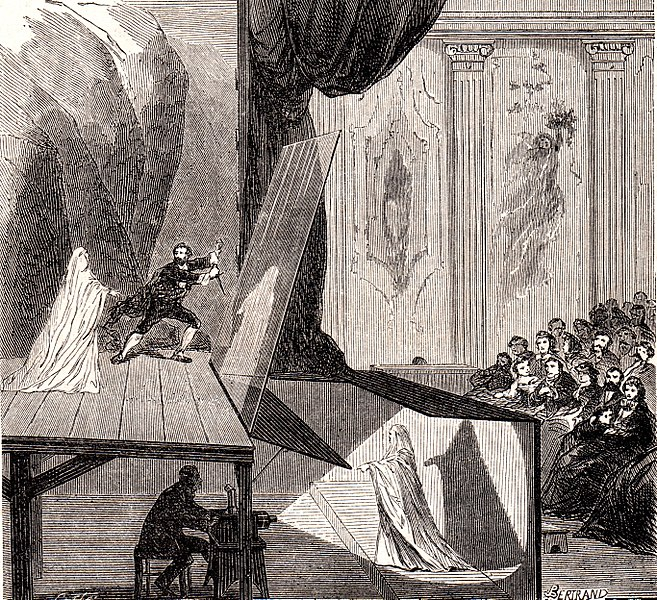
\includegraphics[width=.5\textwidth]{img/Peppers_Ghost.jpg}souce: Wikipedia\\
Jedná se divadelní trik, jež skládá pozorovateli dva obrazy přes sebe a vytváří iluzi
hologramu nebo ducha. Původně byl vyvinut pro divadelní představení, v moderní
době však dokáže simulovat i hologram, který známe ze sci-fi.

\subsubsection{Modely a textury}
Modely jsou z webu https://3dwarehouse.sketchup.com a
textury z webu https://www.textures.com/ a https://texturehaven.com/.\\
V programu blender pak byly tyto textury namapovány na objekt a bylo do nich
zapečeno ambient oclusion (stíny vytvořené stísněným prostorem).

\chapter{instalace a spusteni}

\chapter{Reseni}

\section{vysledny web}

\section{uzivatelska dokumentace}

\chapter*{Závěr}
\noindent
Výsledkem je vytvořená webová aplikace a serverová aplikace poskytující API.
\\


Webová aplikace je podle technologie single-page application,
využívající nejmodernější webové technologie jak na straně uživatele tak i na straně
serveru. Frontend využívá velmi přívětivý design \textit{Material design} a 
poskytuje uživateli přívětivé prostředí pro práci. Zadavatelé zde naleznou
prostředí pro zadávání nových záznamů nekolika druhů, které pak následně
mohou editovat či mazat. Hotové záznamy může kdokoliv prohledávat a
třídit pomocí několika vestavěných parametrů a následně si požadovaný záznam
plně zobrazit. Web obsahuje i redakční systém, který je spravován redaktory,
kteří přidávají články do rubriky novinky a editují obsah webu.
\\


Vedle hlavní frontend aplikace je možné si načíst i oddělené moduly.
První modul poskytuje hologram 3D modelu, který se hodí zejména na výstavy.
Druhý modul přináší interaktivní prohlížení 2D map z Krkonoš 19. století.
\\


Serverová aplikace poskytuje nejen samotnou webovou aplikaci, ale i 
moduly nezávislé na hlavní aplikaci. Ty pak komunikují se serverem pomocí API,
ktere je dobře zdokumentováno a poskytuje tak přístup k datům i pro 
externí programátory a jejich programy.
\\


Do systému bylo uživateli zadáno přes 35000 záznamů různých typů a velikostí.
Samotný web obsahuje mnoho článků, informativních stránek a novinek.


\addcontentsline{toc}{chapter}{Závěr}


%%% Seznam použité literatury
%%% Seznam použité literatury (bibliografie)
%%%
%%% Pro vytváření bibliografie používáme bibTeX. Ten zpracovává
%%% citace v textu (např. makro \cite{...}) a vyhledává k nim literaturu
%%% v souboru literatura.bib.
%%%
%%% Příkaz \bibliographystyle určuje, jakým stylem budou citovány odkazy
%%% v textu. V závorce je název zvoleného souboru .bst. Styly plainnat
%%% a unsrt jsou standardní součástí latexových distribucí. Styl czplainnat
%%% je dodáván s touto šablonou a bibTeX ho hledá v aktuálním adresáři.

\bibliographystyle{czplainnat}    %% Autor (rok) s českými spojkami
% \bibliographystyle{plainnat}    %% Autor (rok) s anglickými spojkami
% \bibliographystyle{unsrt}       %% [číslo]

\renewcommand{\bibname}{Seznam použité literatury}

%%% Vytvoření seznamu literatury. Pozor, pokud jste necitovali ani jednu
%%% položku, seznam se automaticky vynechá.

\bibliography{literatura}

%%% Kdybyste chtěli bibliografii vytvářet ručně (bez bibTeXu), lze to udělat
%%% následovně. V takovém případě se řiďte normou ISO 690 a zvyklostmi v oboru.

% \begin{thebibliography}{99}
%
% \bibitem{lamport94}
%   {\sc Lamport,} Leslie.
%   \emph{\LaTeX: A Document Preparation System}.
%   2. vydání.
%   Massachusetts: Addison Wesley, 1994.
%   ISBN 0-201-52983-1.
%
% \end{thebibliography}


%%% Obrázky v bakalářské práci
%%% (pokud jich je malé množství, obvykle není třeba seznam uvádět)
\listoffigures

%%% Tabulky v bakalářské práci (opět nemusí být nutné uvádět)
%%% U matematických prací může být lepší přemístit seznam tabulek na začátek práce.
\listoftables

%%% Použité zkratky v bakalářské práci (opět nemusí být nutné uvádět)
%%% U matematických prací může být lepší přemístit seznam zkratek na začátek práce.
\chapwithtoc{Seznam použitých zkratek}

%%% Přílohy k bakalářské práci, existují-li. Každá příloha musí být alespoň jednou
%%% odkazována z vlastního textu práce. Přílohy se číslují.
%%%
%%% Do tištěné verze se spíše hodí přílohy, které lze číst a prohlížet (dodatečné
%%% tabulky a grafy, různé textové doplňky, ukázky výstupů z počítačových programů,
%%% apod.). Do elektronické verze se hodí přílohy, které budou spíše používány
%%% v elektronické podobě než čteny (zdrojové kódy programů, datové soubory,
%%% interaktivní grafy apod.). Elektronické přílohy se nahrávají do SISu a lze
%%% je také do práce vložit na CD/DVD. Povolené formáty souborů specifikuje
%%% opatření rektora č. 72/2017.
\appendix
\chapter{Přílohy}

\section{První příloha}

\openright
\end{document}
